%%=============================================================================
%% Methodologie
%%=============================================================================

\chapter{\IfLanguageName{dutch}{Methodologie}{Methodology}}
\label{ch:methodologie}

\section{Type onderzoek}
Het onderzoek beschreven in deze tekst is een \textbf{kwantitatief} onderzoek. Voor combinaties van het aantal auto's en het aantal reservaties zullen het service level, de totale gebruiksduur van de auto's en de tijdsduur van de reservaties die niet konden doorgaan vergeleken worden. Vanuit een bedrijfsstandpunt is het interessant om het service level en de gebruiksduur van de auto's maximaliseren voor een gegeven grootte van de vloot. Voor dit onderzoek wordt geopteerd voor een aanpak die zo dicht mogelijk aansluit bij de realiteit binnen het bestek van het onderzoek. In plaats van de meer theoretische en wiskundige aanpak met wachtrijtheorie beschreven in de stand van zaken worden er in dit onderzoek simulaties uitgevoerd uit met een zelf-ontwikkelde simulatietool. De programmeercode van deze simulatietool is als bijlage opgenomen. Deze simulaties simuleren reëel reservatiegedrag van de Partago gemeenschap en zijn gebaseerd op historische reservaties van Partago. Verder in dit hoofdstuk wordt exact beschreven hoe deze simulaties zijn opgebouwd en welke stappen binnen elke simulatie uitgevoerd worden om tot numerieke waarden voor het service level en de gebruiksduur van de auto's te komen. 

\section{Opzet van een simulatie}
\subsection{Doel}
Tijdens de simulatie wordt er een getracht tweemaal een toewijzing te doen van de beschikbare auto's aan de reservaties in de simulatie. Eenmaal zal deze toewijzing gebeuren op een eenvoudige manier (zie verder) en eenmaal zal deze toewijzing gebeuren door het oplossen van het corresponderende Constraint Satisfaction Problem (zie verder en stand van zaken). Voor beide toewijzingen wordt dan het service level, de tijd dat de auto's actief waren en de tijd van reservaties die niet konden doorgaan omdat er geen auto beschikbaar was berekend. Elke karakteriserende simulatie wordt meermaals uitgevoerd om genoeg datapunten voor de grootheden te genereren. Hierdoor kan per set van karakteristieke parameters een gemiddelde en standaard afwijking berekent worden. 

\subsection{Karakteristieken}
Eén enkele simulatie wordt gekarakteriseerd door waarden van de volgende grootheden:
\begin{itemize}
	\item \textbf{Aantal reservaties in de simulatie:}
	Het aantal reservaties is een maat voor de drukte op het systeem. Het aantal gebruikers van het systeem zou hier geen goede maat voor zijn, weinig gebruikers kunnen immers ook relatief veel reservaties maken. Veel reservaties betekent een grote drukte op het systeem, weinig reservaties betekent een kleine drukte. Uiteraard kunnen overlappende reservaties niet van dezelfde persoon afkomstig zijn. De reservaties gebruikt in de simulatie zijn bestaande historische reservaties van Partago.
	\item \textbf{Aantal auto's:}
	Tijdens de simulatie zullen er toewijzingen gebeuren van de auto's aan de reservaties. Meer auto's beschikbaar in de fictieve zone zal het service level onmiddellijk doen toenemen. Voor eenzelfde aantal reservaties zullen meer reservaties kunnen doorgaan als er meer auto's beschikbaar zijn. 
	\item \textbf{Aantal weken:}
	Elke simulatie stelt een fictieve reserveringsperiode voor van een aantal weken. Tijdens dit onderzoek wordt deze parameter vastgehouden op \textbf{2 weken}. Tijdens elke simulatie zullen we dus een periode van 2 weken simuleren. 
\end{itemize} 

\subsection{Stappen binnen een simulatie}
Binnen één enkele simulatie worden de volgende stappen ondernomen
\begin{enumerate}
	\item Definiëren van de karakteriserende parameters
	\item Historische Partago reservaties ophalen
	\item Een dataset van reservaties genereren op basis van de historische gegevens voor de gedefinieerde periode
	\item Een eenvoudige toewijzing doen van auto's op de reservaties uit de dataset
	\item Een toewijzing doen van auto's op de reservaties uit de dataset met behulp van een CSP oplosalgoritme 
	
\end{enumerate}
Op elk van deze stappen wordt dieper ingegaan in de komende secties van dit hoofdstuk. 

\section{Definiëren van de karakteriserende parameters}
\subsection{Aantal reservaties}
\subsection{Aantal auto's}
\subsection{Aantal weken}
Zoals eerder vermeld zal deze parameter vastgehouden worden op 2 weken. Deze keuze is arbitrair. De simulaties over een langere periode laten lopen zou de rekentijd aanzienlijk verhogen en weinig meerwaarde bieden. Zoals eerder vermeld wordt een simulatie met een set van parameters meermaals uitgevoerd zodat de resultaten uitgemiddeld worden. 

\section{Partago reservaties ophalen}
De dataset van reservaties die gegenereerd wordt is gebaseerd op bestaande reservaties uit het verleden gedaan op het systeem van Partago. Dit geeft als voordeel dat de dataset een reëel karakter zal vertonen en dus dicht aansluit op werkelijk reserveringsgedrag. Voor dit onderzoek worden historische gegevens van Partago van 1 januari 2019 tot en met 30 juni 2019 gebruikt. Voor filtering zijn dit 7661 reservaties die gebruikt kunnen worden om datasets uit te generen. Dit aantal wordt wel nog opgekuist vooraleer de dataset gegenereerd wordt: reservaties niet uitgevoerd door Partago-coöperanten (bijvoorbeeld door het onderhoudsteam), reservaties korter dan 5 minuten, reservaties langer dan 24uur en geannuleerde reservaties worden verwijderd.

\section{Dataset van reservaties genereren}
Uit de gefilterde lijst van Partago reservaties zal een dataset van reservaties gegenereerd worden voor een periode van het gedefinieerde aantal weken. In dit onderzoek zal elke dataset dus bestaan uit reservaties voor 2 weken. De parameter "aantal reservaties" zal bepalen hoeveel reservaties zich in de dataset bevinden. Dit aantal wordt willekeurig geselecteerd uit de historische Partago reservaties en gemapt op een willekeurige week in de dataset (week1 of week2), maar met behoudt van de dag van de week. Reservatiegedrag op een dinsdag is mogelijks niet hetzelfde als reservatiegedrag op een zaterdag. Deze informatie mag dus niet verloren gaan tijdens het mappen. Aangezien de reservaties willekeurig geselecteerd worden zullen de reservaties per dag in een willekeurige volgorde staan. Dit is eveneens de volgorde waarmee de reservaties toekomen bij het systeem. Figuur3.1 is een visuele voorstelling van een eenvoudige dataset van 2 weken met 38 reservaties.
\begin{figure}[h]
	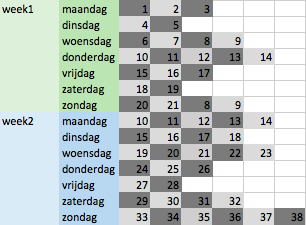
\includegraphics{dataset.png}
	\caption{visuele voorstelling van een dataset}
\end{figure}
\section{Eenvoudige toewijzing}
\section{Toewijzing met behulp van een CSP}





